% Appendix: system parameters and settings referenced from the Methods.
% LoG: submitted after the bibliography. Nature Portfolio: becomes Supplementary Information.
\section{Case-study generators}
\label{app:cases}

\paragraph{Form of dependence.} $M=12$ channels in three blocks of four, $T=2000$. The latent $u$ is a standardised AR(1) process with coefficient $0.8$. Within every block the noise levels $s_i$ are log-spaced on $[0.2, 1]$, so the loading $1/\sqrt{1+s_i^2}$ sets each channel's strength. Maps: linear $g(w)=w$; monotone $g(w)=\sinh(2w)$, odd, so its pairs with folded channels have $r=\rho=0$ in population; fold $g(w)=w^2$. Configurations: all blocks linear; one monotone block; one folded block; one monotone and one folded block. Channels are $z$-scored after the map. SPIs: empirical covariance of the standardised channels (equal to Pearson $r$), Spearman $\rho$, and MI by the Kraskov--St\"ogbauer--Grassberger estimator \will{cite; confirm $k$}. Seed base 20261028.

\paragraph{Timing of dependence.} $M=15$ channels in three blocks of five, $T=1000$. The mother $m$ is an Ornstein--Uhlenbeck process with lag-one autocorrelation $0.9$ on a grid eight times finer than the samples, read by linear interpolation so that fractional delays do not smooth it. Lagged block: constant delays $\{1,2,3,4,5\}$ samples. Warped block: $d_i(t) = A_i \sin(2\pi t/250)$ with $A_i \in \{2,4,6,8,10\}$ samples. Observation noise $\sigma_i$ is log-spaced on $[0.1, 0.4]$ and assigned in the fixed order $(1,4,2,0,3)$ within each block, so noise does not follow lag or warp. Random draws do not depend on the block layout, so a channel whose block kind is unchanged is identical across configurations. SPIs: normalised Euclidean distance; cross-pairwise Euclidean distance, minimised over shifts up to 250 samples; unconstrained, normalised DTW. Seed base 20261029.

\section{Generative classes}
\label{app:proof}
$M \in \{8,16,32\}$, $T \in \{500,1000,2000\}$, ten instances per cell; full benchmarked catalogue \will{$K$}. VAR weights are literal: $\phi$ on self, the stated coupling on each of the two ring neighbours, so both VAR variants have total weight $0.9$.

\begin{table}[ht]
	\centering
	\caption{\textbf{Generative classes.} \will{Add generator equations; check against the proof configuration.}}
	\label{tab:classes}
	\small
	\rowcolors{2}{white}{tablestripe}
	\begin{tabularx}{\linewidth}{@{} l l >{\raggedright\arraybackslash}X @{}}
		\toprule
		\rowcolor{tableheader}
		\textbf{Family} & \textbf{Variant} & \textbf{Parameters} \\
		\midrule
		Noise & Gaussian & independent channels \\
		Noise & Cauchy & independent channels \\
		VAR & self-memory & ring, $\phi = 0.7$, neighbour coupling $0.1$ each side \\
		VAR & neighbour coupling & ring, $\phi = 0.2$, neighbour coupling $0.35$ each side \\
		Kuramoto & fast frequencies & all-to-all, $K=-4$, $\bar{\omega} = 3$, $\mathrm{sd}(\omega) = \sqrt{3}$, $\mathrm{d}t = 0.00625$ \\
		Kuramoto & slow frequencies & as above, $\bar{\omega} = 0.025$, $\mathrm{sd}(\omega) = 0.0144$ \\
		CML & intermittency & quadratic map, $\alpha = 1.7522$, $\varepsilon = 0.00115$ \\
		CML & developed turbulence & quadratic map, $\alpha = 2$, $\varepsilon = 0.3$ \\
		Wave equation & 1-D & periodic lattice, $c = 10$, five initial modes (decay $1.5$), noise sd $0.01$ \\
		\bottomrule
	\end{tabularx}
\end{table}

\paragraph{Embedding and coordinates.} t-SNE by openTSNE 1.0.4: perplexity 30, Student-$t$ kernel with five degrees of freedom, PCA initialisation, Euclidean metric, early exaggeration 12 for 250 iterations, 1250 iterations, seed 260924 \will{state the input: missing-value handling, scaling}. Separability: five-nearest-neighbour classification on the leading 50 principal components, each $(M,T)$ cell held out in turn. Raincloud coordinates: chosen among those with training AUC $\geq 0.995$ in every $(M,T)$ cell on instances 0--5; distributions show instances 6--9.

\paragraph{Intermittency recordings near noise.} Two of the 90 intermittency recordings embed with Gaussian noise (\cref{fig:proof}a); they are the only two errors of the nearest-neighbour check. Both are 8-site windows of a 100-site lattice that, as a whole, alternates between laminar and turbulent domains as intermittency should, and each window caught one extreme of the regime (\cref{fig:strays}). In one ($T=1000$), all eight sites stay on the same period-3 laminar orbit throughout, so every channel carries the same signal. Dependence is maximal, but every pair of channels is alike, and $z$, a correlation across pairs, has nothing to read. 56 of the 225 statistics do not vary across pairs, leaving 46\% of $z$ undefined; on the coordinates that remain, its ten nearest neighbours are all Gaussian noise, so the filled-in values do not place it there. Windows that are 97--99\% laminar approach the same boundary; the 99\% window, in which one site bursts 5\% of the time, stays in its island. In the other ($T=500$), the window sits on a turbulent domain that persists for the whole record. Its dependence is weak and nearly uniform across pairs, and at this size it does not rise above estimation noise: an equally weak window at $T=2000$ stays in its island, as do developed-turbulence recordings with weaker dependence at larger $M$. The two recordings lie at opposite extremes of dependence strength yet land together, so their position reflects the absence of a contrast between pairs, not the strength of dependence. $z$ alone cannot separate such recordings from noise; their dependence strengths can.

\begin{figure}[ht]
	\centering
	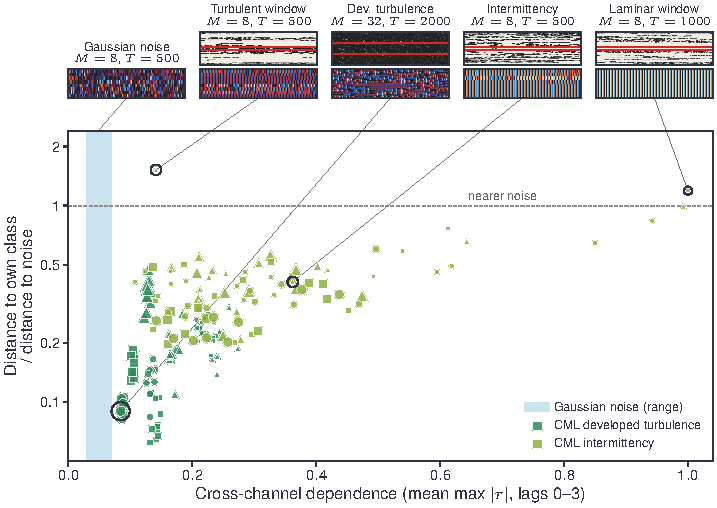
\includegraphics[width=0.7\linewidth]{proof-strays}
	\caption{\textbf{Two intermittency recordings embed with noise for opposite reasons.} Every intermittency and developed-turbulence recording of \cref{fig:proof}, by cross-channel dependence (mean over ordered channel pairs of the largest $|r|$ at lags 0--3) against its distance to its own class median divided by its distance to the Gaussian-noise median, on the leading 50 principal components; above the dashed line a recording is nearer noise. Marker area encodes $M$ and shape encodes $T$, as in \cref{fig:proof}; the shaded band spans Gaussian noise. Insets, for the circled recordings: the full 100-site lattice over the whole record (black: turbulent, $|x_t - x_{t-3}| \geq 0.05$), observed sites boxed in red, above the first 120 steps of the observed window; the Gaussian-noise inset shows one recording.}
	\label{fig:strays}
\end{figure}

\section{Order-parameter systems}
\label{app:order}
\will{One paragraph per system: model, control parameter and sweep, observation (which variables, $M$, $T$), definition of $Q$, development/held-out split. Systems: cross-frequency 2:1 locking ($M=N=24$); electronic-oscillator hardware recordings; Stuart--Landau oscillators ($M=N=32$, $T=1000$, $K=0.8$, $\gamma \in [0.68, 0.77]$); two-dimensional coupled map lattice ($L=256$, $g=0.2$, $M=32$ dispersed sites, $T=1000$).}
